\documentclass{article}\usepackage[]{graphicx}\usepackage[]{color}

\usepackage{alltt}
\usepackage{float}
\usepackage{graphicx}
\usepackage{tabularx}
\usepackage{siunitx}
\usepackage{amssymb} % for math symbols
\usepackage{amsmath} % for aligning equations
\usepackage{textcomp}
\usepackage{booktabs}
\usepackage{mdframed}
\usepackage{natbib}
\usepackage{comment}
\usepackage{booktabs}
\usepackage[colorinlistoftodos]{todonotes} % to make comments on the margin
\usepackage[small]{caption}
\setlength{\captionmargin}{30pt}
\setlength{\abovecaptionskip}{0pt}
\setlength{\belowcaptionskip}{10pt}
\topmargin -1.5cm        
\oddsidemargin -0.04cm   
\evensidemargin -0.04cm
\textwidth 16.59cm
\textheight 21.94cm 
%\pagestyle{empty} %comment if want page numbers
\parskip 7.2pt
\renewcommand{\baselinestretch}{1.5}
\parindent 0pt
%\usepackage{lineno}
%\linenumbers

%% R Script

\title{Unravelling the phenology-phylogeny tangle.}

% alternative titles:
%% An expanded bayesian phylogenetic mixed model to unravel the phenology-phylogeny tangle. %% this sounds too methodsy

\begin{document}

\maketitle

\noindent Authors:\\
The Wolkovich Lab in 2019 \& collaborators $^{1,2,3,4}$ % Will Pearse, Jonathan Davies also
\vspace{2ex}\\
\emph{Author affiliations:}\\
$^{1}$Forest \& Conservation Sciences, Faculty of Forestry, University of British Columbia, 2424 Main Mall, Vancouver, BC V6T 1Z4;\\
$^{2}$Arnold Arboretum of Harvard University, 1300 Centre Street, Boston, Massachusetts, USA;\\
$^{3}$Organismic \& Evolutionary Biology, Harvard University, 26 Oxford Street, Cambridge, Massachusetts, USA;\\
$^{4}$Edificio Ciencias, Campus Universitario 28805 Alcalá de Henares, Madrid, Spain\\
 

\vspace{2ex}
$^*$Corresponding author: ignacio.moralesc@uah.es\\
\renewcommand{\thetable}{\arabic{table}}
\renewcommand{\thefigure}{\arabic{figure}}
\renewcommand{\labelitemi}{$-$}
\setkeys{Gin}{width=0.8\textwidth}

%%%%%%%%%%%%%%%%%%%%%%%%%%%%%%%%%%%%%%%%%%%%%%%
%%%%%%%%%%%%%%%%%%%%%%%%%%%%%%%%%%%%%%%%%%%%%%%
\clearpage



%%%%%%%%%%%%%%%%%%%%%%%%%%%%%%%
% Results & Discussion
%%%%%%%%%%%%%%%%%%%%%%%%%%%%%%%

%%%%%%%%%%%%%%%%%%%%%%%%%%%%%%%
% Discussion
%%%%%%%%%%%%%%%%%%%%%%%%%%%%%%%

%\section*{Discussion}
% EMW (26Apr2022): Some great text here! Would flow really well with a combined R&D.
%IMC 06may - Giving a try at merging Results and Discussion below


\section*{Results \& Discussion}

Most analyzed species were sensitive to all three environmental cues---i.e., forcing, chilling, and photoperiod (Figs. \ref{fig:muplot_all}, Supporting Table \ref{tab:}). Cue sensitivity led to phenological advances of 7.2 days per unit of standardized chilling, 5.8 days per unit of forcing, and 1.4 days/standard unit of photoperiod (see Table \ref{tab:modelanglamb}), on average. These average sensitivities to cues vary widely across species with larger variation found in species' responses to chilling, then to forcing and very little variation in how  species respond to photoperiod (Figs. \ref{fig:muplot_all}, Supporting Table \ref{tab:}). Overall, these findings coincide in their ranking of cue importance with previous ones \citep{ettinger2020}.\\

Our results reveal how responses to cues greatly differ among clades. For example, oaks and beeches (Fagaceae), elms (Ulmaceae) and buckthorns (Rhamnaceae) are highly sensitive to chilling while rhododendrons (Ericaceae), butterfly bushes (Scrophulariaceae) or spindles (Celastraceae) show little to no response to chilling (Fig. \ref{fig:muplot_all} a). %IMC: not sure if we need some natural history here or some mention to research for some of these clades. Lizzie, if you want to mention-cite something here, please jump in.
A similar clade-level variation is found for forcing, where some of these clades---e.g., Ericaceae, Rhamnaceae, Ulmaceae, or Fagaceae---are particularly sensitive (advancing their budburst more than 10 days per standardized unit of forcing) and others such as the Sapindaceae, Cornaceae or Juglandaceae families show little response (Fig. \ref{fig:muplot_all} b).\\ 

Considering more than one cue, some clades are highly sensitive to two cues at the same time, which would suggest the existance of syndromes where the genetic basis for responses to one cue (e.g., forcing) could have been selected for along responses to another cue (e.g. chilling). However, clade-level responses to multiple cues are significantly but weakly correlated (\emph{r} = 0.31; between forcing an chilling) as responses to chilling are more variable and, the relationship among responses is non-linear (see Supporting Information XX). Weak correlations likely reflect how other clades such as \emph{Tilia} and Ericaceae display strong responses to forcing but weak responses to chilling, or how genera such as \emph{Betula} and \emph{Populus} show strong intra-clade differences in their responses to chilling (Fig. \ref{fig:muplot_all}). Interestingly, whichever the type of response, phenological responses to cues show structuring at the clade level that could have an evolutionary imprint in the phylogeny. % I don't love this last sentence, but was trying to find a way to connect with phylogenetic results coming next.
\\

Our modelling approach allows to explicitly test whether there is phylogenetic structuring in how species respond to environmental cues. Phylogenetic signal as measured by our `phylogenetic shrinkage parameter' ($\lambda$) differs markedly across cues (Fig. \ref{fig:phylosig_all}). Tree phenological responses to environmental cues were strongly phylogenetically clustered for forcing ($\lambda = 0.65$), moderately so for chilling ($\lambda = 0.54$) and weakly for photoperiod ($\lambda= 0.39$) (see Fig. \ref{Fig:muplot_all}, Table \ref{tab:modelanglamb}). Sensitivity to photoperiod treatments did not vary across clades while responses to forcing tend to be more similar among closely related species (Fig. \ref{fig:muplot_all}). Results showing that closely related species tend to show similar responses to some cues but not others, support the need to account for phylogeny in multi-species, multi-predictor modelling of phenological responses to cues.\\

Along evolution, tree species would have been constrained % I'm aware the term constrained is contentious in this context, so perhaps we can use something else
in their ability to develop responses to forcing that differ much from those of their close relatives, and somewhat less constrained in their responses to chilling. In contrast, responses to photoperiod seem evolutionarily labile, with little variation across most species (0.86 days per standard unit of photoperiod) and a few exceptions from the genus \emph{Fagus}, known as particularly sensitive to photoperiod \citep{fu2019}. Specifically, \emph{Fagus sylvatica} is nearly five times more sensitive to photoperiod than most tree species. The question arises as to whether species with outlying responses should be chosen as the model from which to extrapolate knowledge as done with \emph{Fagus sylvatica} in the phenology literature (REFs for PEP75?!) %HELP with references on Fagus would be appreciated.
.\\

Why would distantly related species respond more similarly and less variably to photoperiod than they do to forcing or chilling? Clearly, daylength is a more 'reliable' cue in temperate latitudes, as it varies (and has varied) less than forcing or chilling both across years and along evolutionary time. As such, it would have enabled species scheduling their phenological events to match most suitable environmental conditions \citep{jackson2009plant}. The adaptation to shifting daylength may have occurred very early in the evolution of photoperiodic sensing---i.e., as early as in cianobacteria \citep{hut2011evolution, serrano2017evolution}. If responses to photoperiod had evolved early in plants and kept more or less constant afterwards in absence of novel selective advantages---i.e., consistent with an Early Burst model of evolution---that would be consistent with our pattern of little variation in the responses to photoperiod across species and clades. Such degree of variation would be measured by our cue-level $\sigma$ parameter, and is significantly smaller for photoperiod than for other cues. We run simulation tests that show how our results for photoperiodic responses would be consistent with the outcome of an Early Burst model of evolution (see Appendix XXX).\\  
% IMC (19NOV22) this last bit of the paragraph needs help from Jonathan and Lizzie to explain a bit what we found in the simulations for delta. Not sure what degree of detail do we need for this in the main text.


From a statistical perspective, accounting for the effects of phylogenetic structuring on the effects of jointly modelled cues had an effect on model coefficients (Fig. \ref{fig:correls_angio}). Not accounting for phylogeny (or assuming $\lambda$ = 0) biased model coefficients, particularly so for forcing and somewhat less for chilling (Fig. \ref{fig:correls_angio}). Specifically, species sensitivities to forcing and chilling were underestimated on average (model slopes shifted by 7.2\% and 3.7\%, respectively). Sensitivities to photoperiod, which showed weak phylogenetic signal were not biased in non-phylogenetic models (Fig. \ref{fig:correls_angio}), likely associated to their low estimated $\lambda$ values. Model intercepts were not affected either (Fig. \ref{fig:correls_angio}).\\ 


Not accounting for phylogeny also had an effect in decreasing cross-species variance in their responses to forcing (Var $\beta_{phylo}$ = 8.74; Var $\beta_{non-phylo}$ = 5.01), chilling (Var $\beta_{phylo}$ = 23.45; Var $\beta_{non-phylo}$ = 17.47), and a smaller effect in increasing variance to photoperiod responses (Var $\beta_{phylo}$ = 0.82; Var $\beta_{non-phylo}$ = 0.93). Counterintuitively, induced reductions in cross-species variance, far from increasing estimation accuracy could lead to increased type-II error by failing to detect actual relationships among cue responses that would only emerge clearly when phylogeny is accounted for (see Supporting Information XX). For example, the correlation between species responses to forcing and chilling decreased by 50\% when model lambda was equal zero (e.g. $r_{force-chill}$ = XX). Importantly, not accounting for phylogeny increased the uncertainty around each individual species estimation of their responses to forcing and chilling (see Fig. SXX in Supporting Information), which could lead to less precise predictions and forecasts of phenology.\\
%IMC: I think this paragraph could use some supervision by Will, to double-check we are not running into any major conceptual mistakes here.

%%%%%%%%%%-------------------- this is where I'm leaving it for today. More tomorrow morning.

%this next paragraph needs shortening, I think we may not need so much detail on lambda =1 model.
Assuming phylogenetic structuring to follow a Brownian Model of evolution ($\lambda$ = 1) biased model coefficients too (Fig. \ref{fig:correls_angio}) although in the opposite direction. Doing so overestimated sensitivities to forcing and chilling (model slopes shifted by 20.5\% and 11.8\%, respectively) and even more to photoperiod (model slopes shifts of 33.1\%; Fig. \ref{fig:correls_angio}). Bias in model coefficients due to either ignoring or overestimating phylogenetic structuring of predictors seems to correlate with the estimated value of $\lambda$ so that, if their actual value is high, coefficients may suffer stronger bias if phylogeny is disregarded. In contrast, if predictor's $\lambda$ is actually low, bias would arise by imposing a Brownian Motion on the evolution of those predictors. Results coincided qualitatively with those of gymnosperms, which were more variable as sample size is smaller (Fig. \ref{fig:correls_angio}). Beyond leading to coefficient shifts, overestimation of phylogenetic structuring of predictors significantly decreased model accuracy---i.e., Bayes$R^{2}$---in both angiosperms (1\%) and gymnosperms (3\%). Ignoring phylogeny did not affect accuracy with respect to our approach (see Appendix XX in Supporting Information).\\ 

Our models found non-negligible phylogenetic signal in model intercepts (see \ref{fig:phylosig_all}). This indicates that the intrinsic variation across species in the timing of budbreak before experiencing the effects of any environmental cue, is also phylogenetically patterned. This is, regardless the action of cues some tree species budbreak earlier than others, and these differences tend to be smaller, at least to some extent (the signal is weak $\lambda$ = 0.35), among closely related species. Previous work had already shown large variation across species in their model intercepts \citep{davies2013phylogenetic}. % not sure this is the right citation, ask Lizzie. This whole paragraph needs work (based on conversation over coffee May6th)  
While fitted species-level intercepts did not change between the phylogenetic and non-phylogenetic model (\ref{fig:correls_angio}), our approach suggests that the mechanisms underlying species' baseline phenological differences would not operate randomly across the phylogeny.\\    

Accurate forecasts of phenology remain elusive, partly due to recent records of declines in species phenological sensitivity to increasing temperatures \citep{fu2015,piao2017}---although such declines could derive from statistical artifacts \citep{wolkovich2021simple}. Whatever the case, tests of declines in phenological sensitivity to warming will rely in accurate estimation of responses to cues, and we show here that such estimations are improved by accounting for phylogenetic relationships. The need to incorporate phylogenetic information into the phenology research programme has been suggested before \citep{davies2013phylogenetic,joly2019importance}, mostly grounded on findings of non-random phylogenetic signal in both phenological traits \citep{davies2013phylogenetic,rafferty2017global} and phenological responses to cues \citep{davies2013phylogenetic,joly2019importance}. Yet, our approach differs from previous research in that it estimates simultaneously phylogenetic signal for each environmental cue driving phenological sensitivity to such cues. Doing so provides insights on how responses to cues have configured along evolutionary time---e.g., if such responses have evolved independently or in concert with each other, and/or if they tend to be shared within certain clades.\\ 


Identifying strong patterns in clade-level responses to cues may open (at least for clades with the strongest signal) a venue for imputation of phenological sensitivities in unmeasured species. Imputation must be done with extreme care \citep{molina2018assessing}, but would allow expanding the short list of plant species for which forecasting phenology is feasible. In any case, the above results have implications for future analyses of phenological responses to cues as they support use of species complexes as done in \cite{ettinger2020}, given the strong structuring of closely related species.\\ %IMC(may22): This paragraph could use some heavy editing to be shortened.



Ultimately, this knowledge would inform which clades will be more sensitive to specific climate shifts---e.g., changes in cold temperatures over winter or in warm temperatures in spring and summer---or, which clades emerge as particularly sensitive to cues only after phylogeny is accounted for. For example, the genus \emph{Quercus} would not be amongst the most sensitive ones to forcing and chilling in non-phylogenetic models (see e.g., \citep{ettinger2020}), but its species gain sensitivity (2 days per standard unit of forcing and 4 days per standard unit of chilling, on average) through the phylogenetic Bayesian models used here.\\ %IMC(20May22): This paragraph needs work

In sum, non-phylogenetic models can (i) induce significant bias in estimated model coefficients, (ii) decrease variability in cross-species biological responses and, (iii) increase  uncertainty around estimates of individual species sensitivity to cues. Further, non-phylogenetic models hide information on whether the evolution of species responses---i.e., phenological shift in our case---to their determining environmental cues has occurred in a correlated fashion, and if so, identifying which clades are more likely to respond in concert to a set of cues (see Fig. \ref{fig:muplot_all}). Together, our results indicate that either ignoring the phylogeny or imposing stronger phylogenetic relationships than actual ones would compromise model ability to generate accurate inference and prediction, which are increasingly needed in a warming world.\\ 


%\subsection*{Model accuracy}
%IMCapr25 - I'd like to include a little subsection here on model accuracy, comparing R2s, LOO, or something similar for our models. Unfortunately, I can't find an easy way to do that (for stanfit objects: https://discourse.mc-stan.org/t/best-way-to-do-prediction-on-new-data-r-rstan-stanfit/1772/17) any help with this is much appreciated. 
% EMW (26Apr2022): To use loo we just need a generated quantities block, right? If so I can try to help code that with Deirdre.
%IMCmay10- I re-run models storing yhats as a generated quantity, and with that computed a Bayes version of R2. There's not change in accuracy between our approach and the lambda0 approach, but accuracy drops if lambda is forced to be equal1. 

%angio
%R2lamb0 0.666
%R2lambest 0.665
%R2lamb1 0.657

%gymno
%R2lamb0 0.527
%R2lambest 0.530
%R2lamb1 0.498



%\item How can we interpret lambdas and sigmas for each cue, and for the intercept?
%\item What are the implications for phenological predictions and forecasts?
%\item Is this approach transferable to different taxa or biological responses? 
%\item Do results differ from what would be expected if single cues where analyzed separately, phylo or non-phylogenetically?


%\item If so, can accounting for phylogeny shed light on the ongoing debate on declining sensitivities? For example, if particular lineages have very different evolutionary constraints on their responses to the cues, they may also display very differt declines in their sensitivities to the cues. % lizzie, I realize I missed important bits on the discussion we had on the relevance of this point, any pointers here are super welcome. 




%\begin{enumerate}
%\item Random discussion points with no home, yet ... 
%\begin{enumerate}
%\item This is a case where phylogeny makes a big difference! Changes overall forcing cues? 
% IMC May6 - sort of dealt with 
%\item Reduced uncertainty in species estimates (I think?) with including phylogeny (goes with above point perhaps also) / % IMC May18 - sort of dealt with 
%\item Even with phylogeny added FagSyl is still freakish for photoperiod cue ... suggesting we've been studying an extreme species as one of our focal species (maybe?) % IMC May18 - this has been dealt with shortly in line 384 (one sentence or so) 
%\item Implications for the declining sensitivities debate? % IMC May18 - done but needs some more work
%\item Highlight/discuss the advantages of pushing methodologies such as the one here % IMC May18 - done but needs some more work



\end{enumerate}
\end{enumerate}

\begin{comment} % I'm pasting this bit from previous version of the intro in case we want to reuse some.
% \item most efforts are on the phenotype rather than on the magnitude of species phenological responsiveness to different environmental cues. 
% Could try to integrate this point above into above paragraph or include in below section that I have commented out ... I think the intro is likely long enough without the below and many of the points could fit in discussion, but up to you!
\iffalse
\item Focused on flowering (and leafout some) times and shifts in them (but see \cite{joly2019importance}, and add REFs!! on other phenological stages: budburst, ripening)
\item Studied trait correlation \citep{bolmgren2008time} (not a limitation, but a different focus)
\item Studied different evolutionary models best fitting the data \citep{rafferty2017global}
\item measured shifts based on field observation data for both climate and phenology (when slopes are available, they represent shifts with time, not shifts with the environment).
\fi
\end{comment}


\bibliography{phylorefs}
\bibliographystyle{amnat}

%%%%%%%%%%%%%%%%%%%%%%%%%%%%%%%
% Tables and Figures
%%%%%%%%%%%%%%%%%%%%%%%%%%%%%%%
\section*{Tables and Figures} 


%IMC 22mar - we should decide among one of the next two figures, instead of having separate figures per cues?
% EMW (28Mar2022): I vote for the first one, but both are great!
\begin{figure} [H]
  \begin{center}
  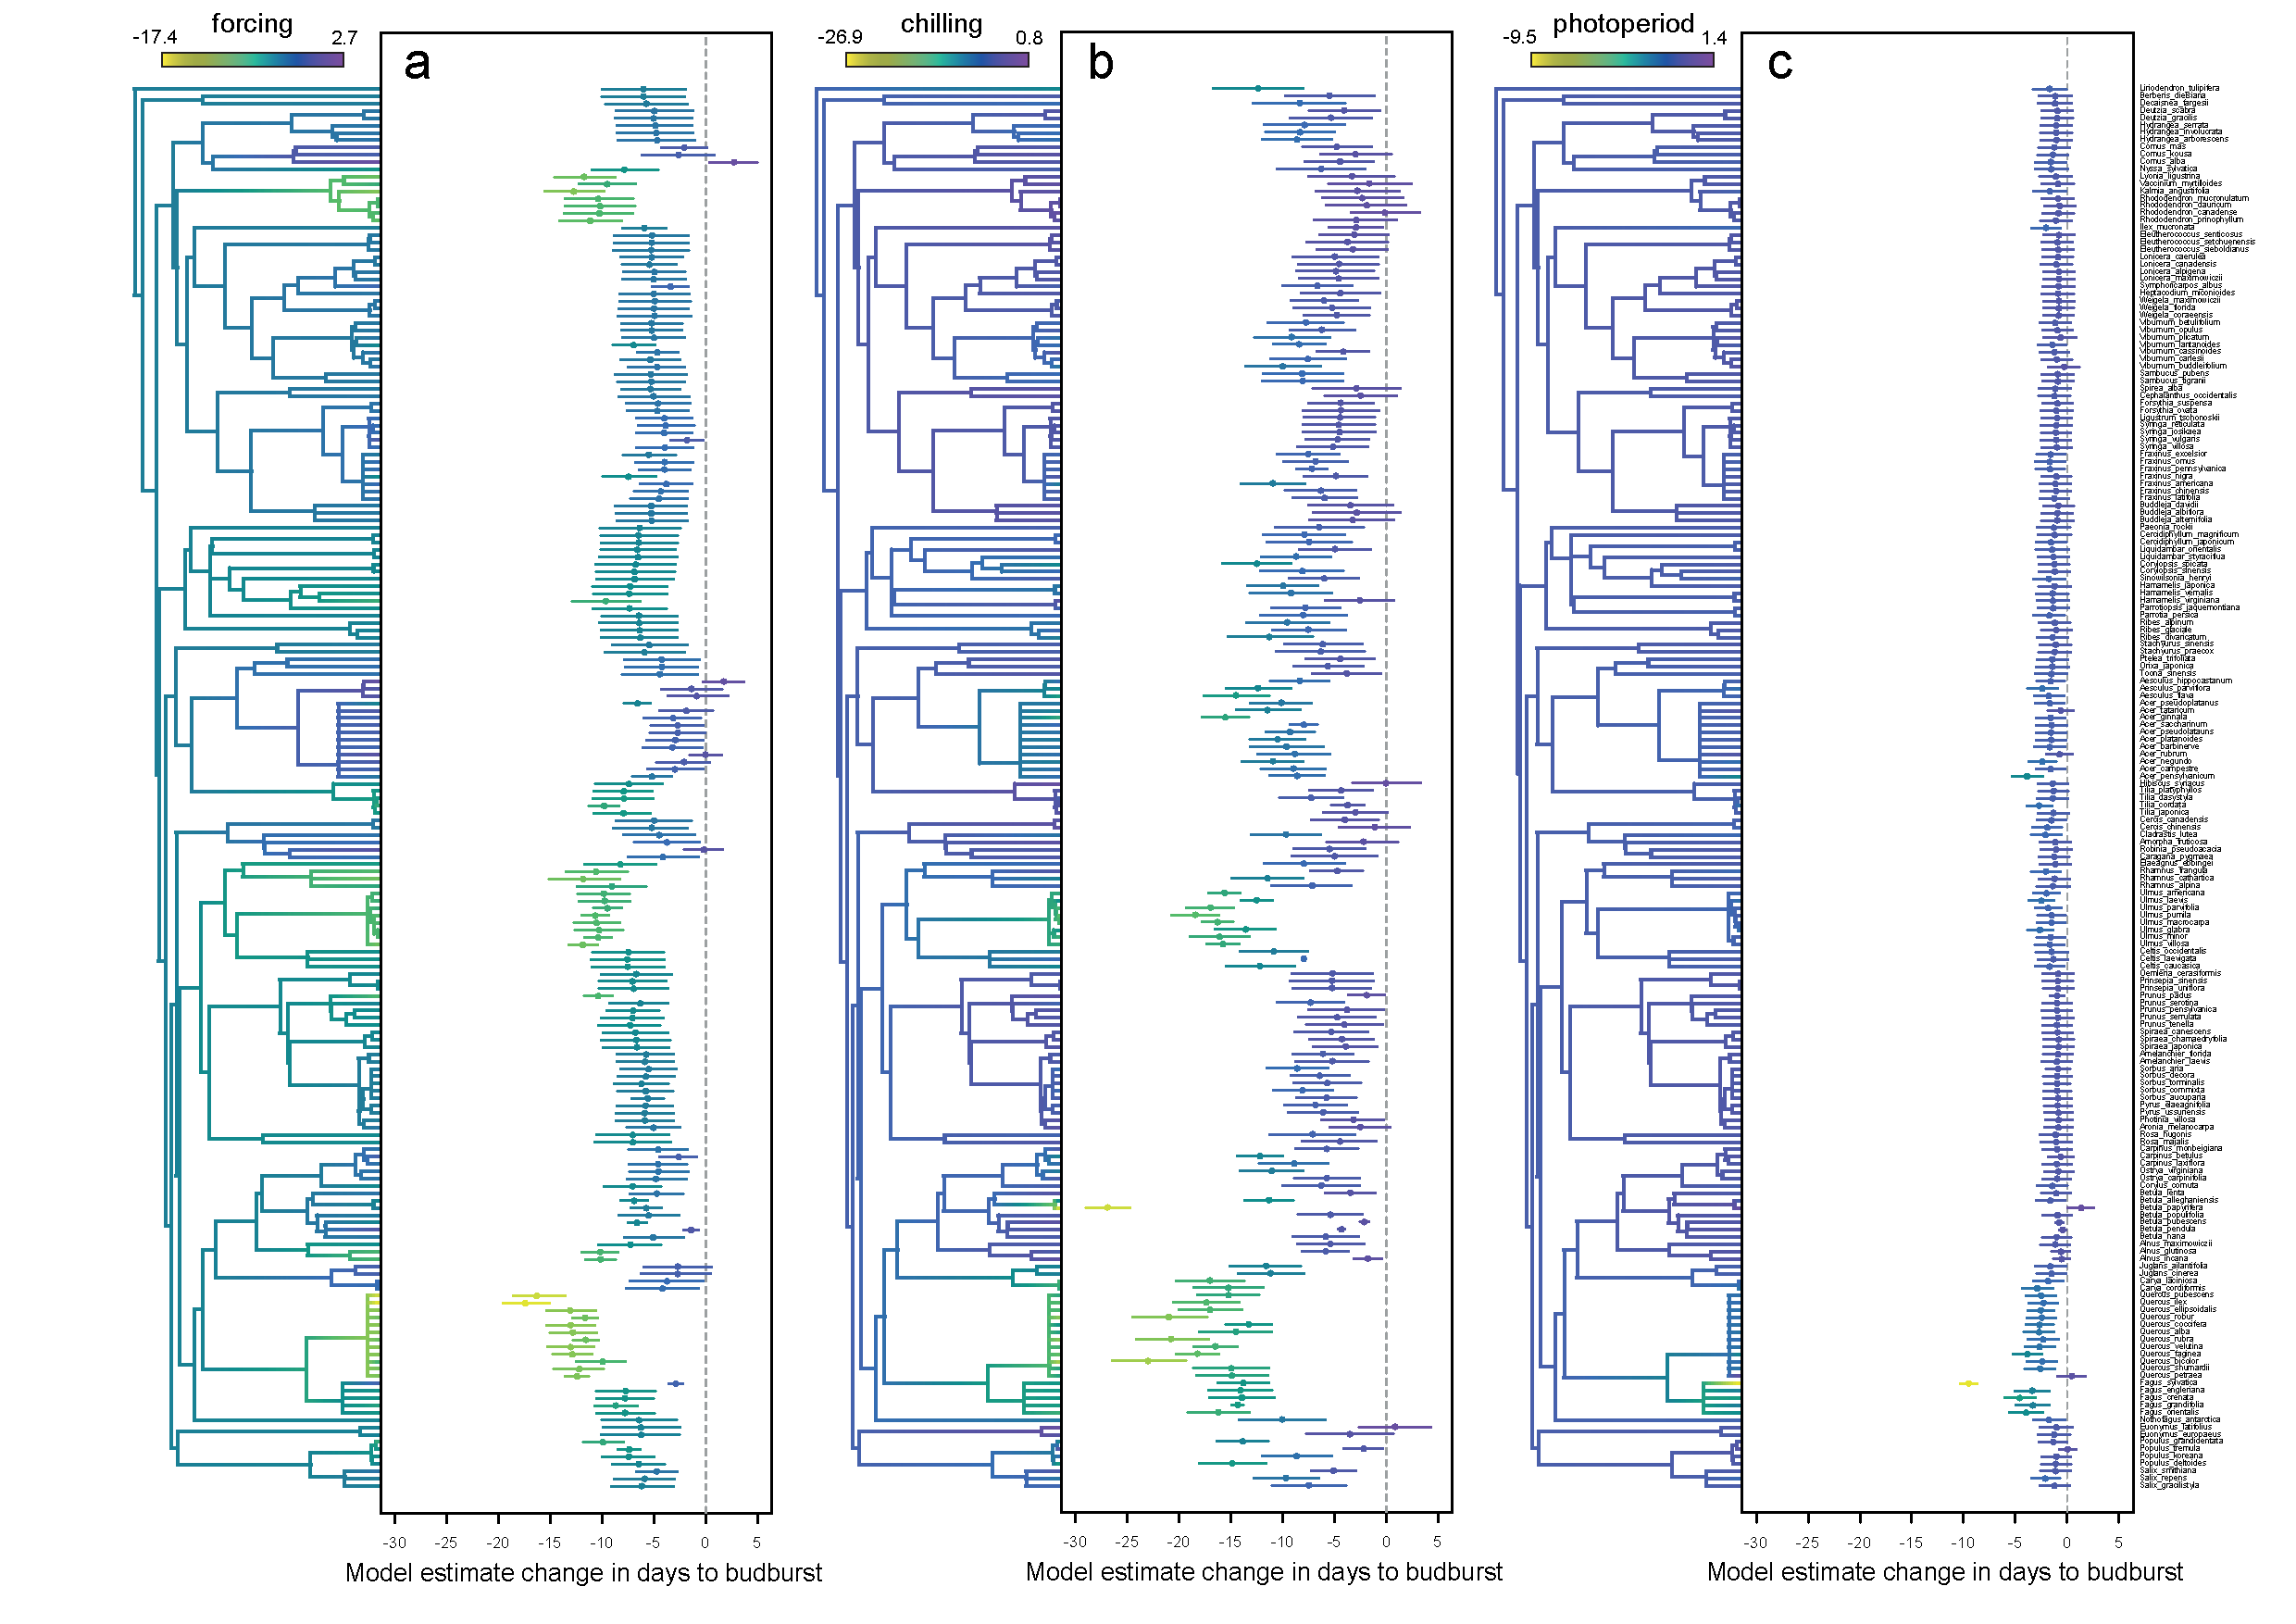
\includegraphics[width=16cm]{../../analyses/phylogeny/figures/muplot_phylo_allcue_angio.pdf}
  \caption{Phenological sensitivity to thee environmental cues, forcing (a), chilling (b) and photoperiod (c) measured in change in days to budburst per standardized unit (z-transformation) of the cues across 192 angiosperm species. The same phylogenetic tree is shown in each panel, colored acording to an estimation of ancestral character states, being the states at the tips the model slopes of our hierarchical phylogenetic model. Note that the color scale varies in each panel. Total tree depth is 81. My.}
  \label{fig:muplot_all}
  \end{center}
\end{figure}

\begin{figure} [H]
  \begin{center}
  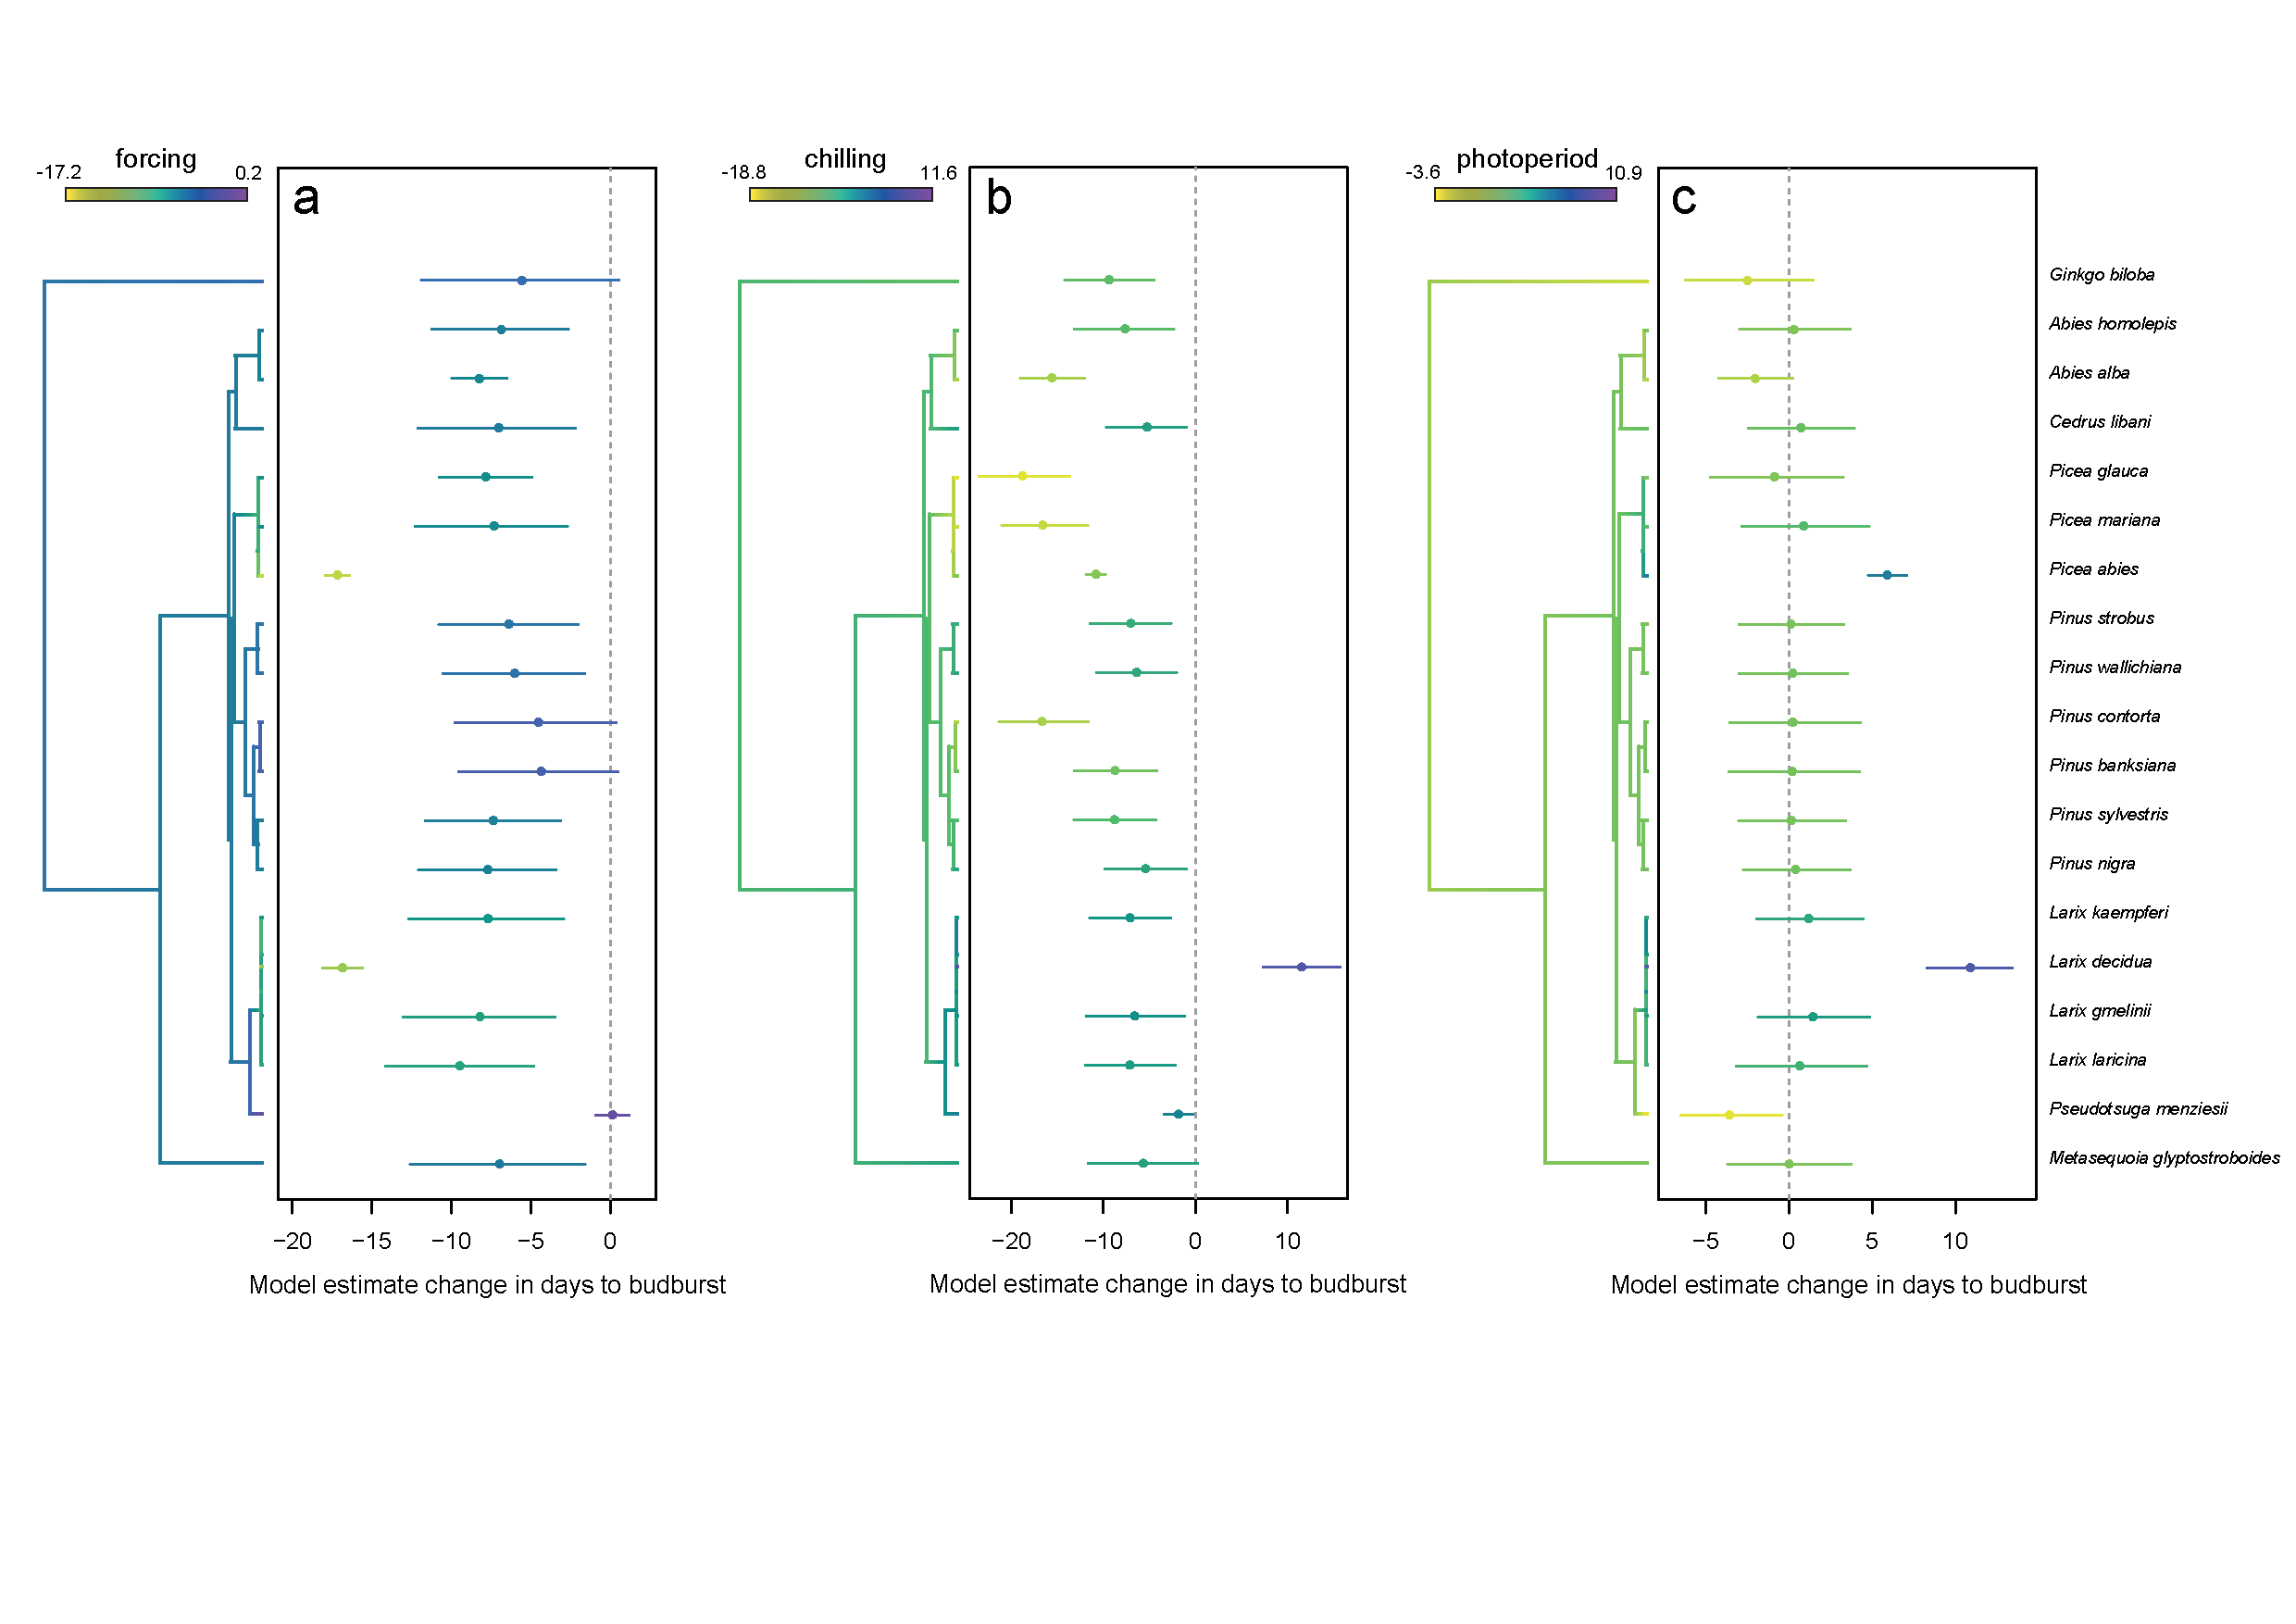
\includegraphics[width=16cm]{../../analyses/phylogeny/figures/Fig1b_phylo_muplots_gymno.pdf}
  \caption{Phenological sensitivity to thee environmental cues, forcing (a), chilling (b) and photoperiod (c) measured in change in days to budburst per standardized unit (z-transformation) of the cues across 19 gymnosperm species. The same phylogenetic tree is shown in each panel, colored acording to an estimation of ancestral character states, being the states at the tips the model slopes of our hierarchical phylogenetic model. Note that the color scale varies in each panel. Total tree depth is 81. My.}
  \label{fig:muplot_allgymno}
  \end{center}
\end{figure}


\begin{figure} [H]
  \begin{center}
  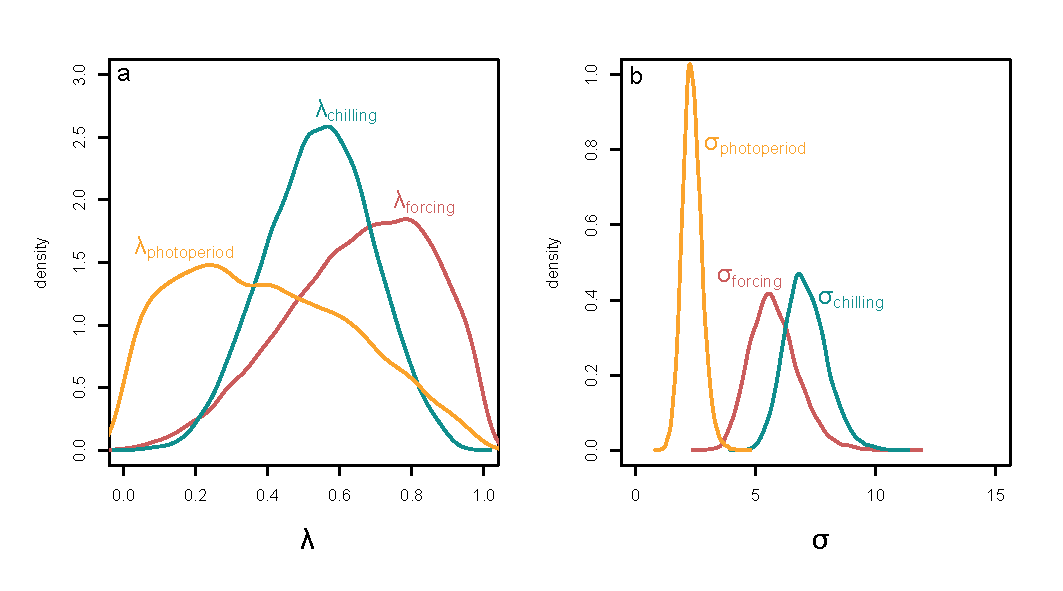
\includegraphics[width=14cm]{../../analyses/phylogeny/figures/Fig2_lambdas_sigmas.pdf}
  \caption{Density plots for the posterior distribution of phylogenetic signal measured by lambda for each cue included as a predictor in the model for angiosperms: forcing (red), chilling (blue),  photoperiod (orange) and for the model intercept (grey). Panels correspond to angiosperms (a-d) and gymnosperms (e-h). Note that lambda estimations corresponding to  panels c-d and g-h as they are constrained to be either equal zero or equal 1.}
  \label{fig:phylosig_all}
  \end{center}
\end{figure}

\begin{figure} [H]
  \begin{center}
  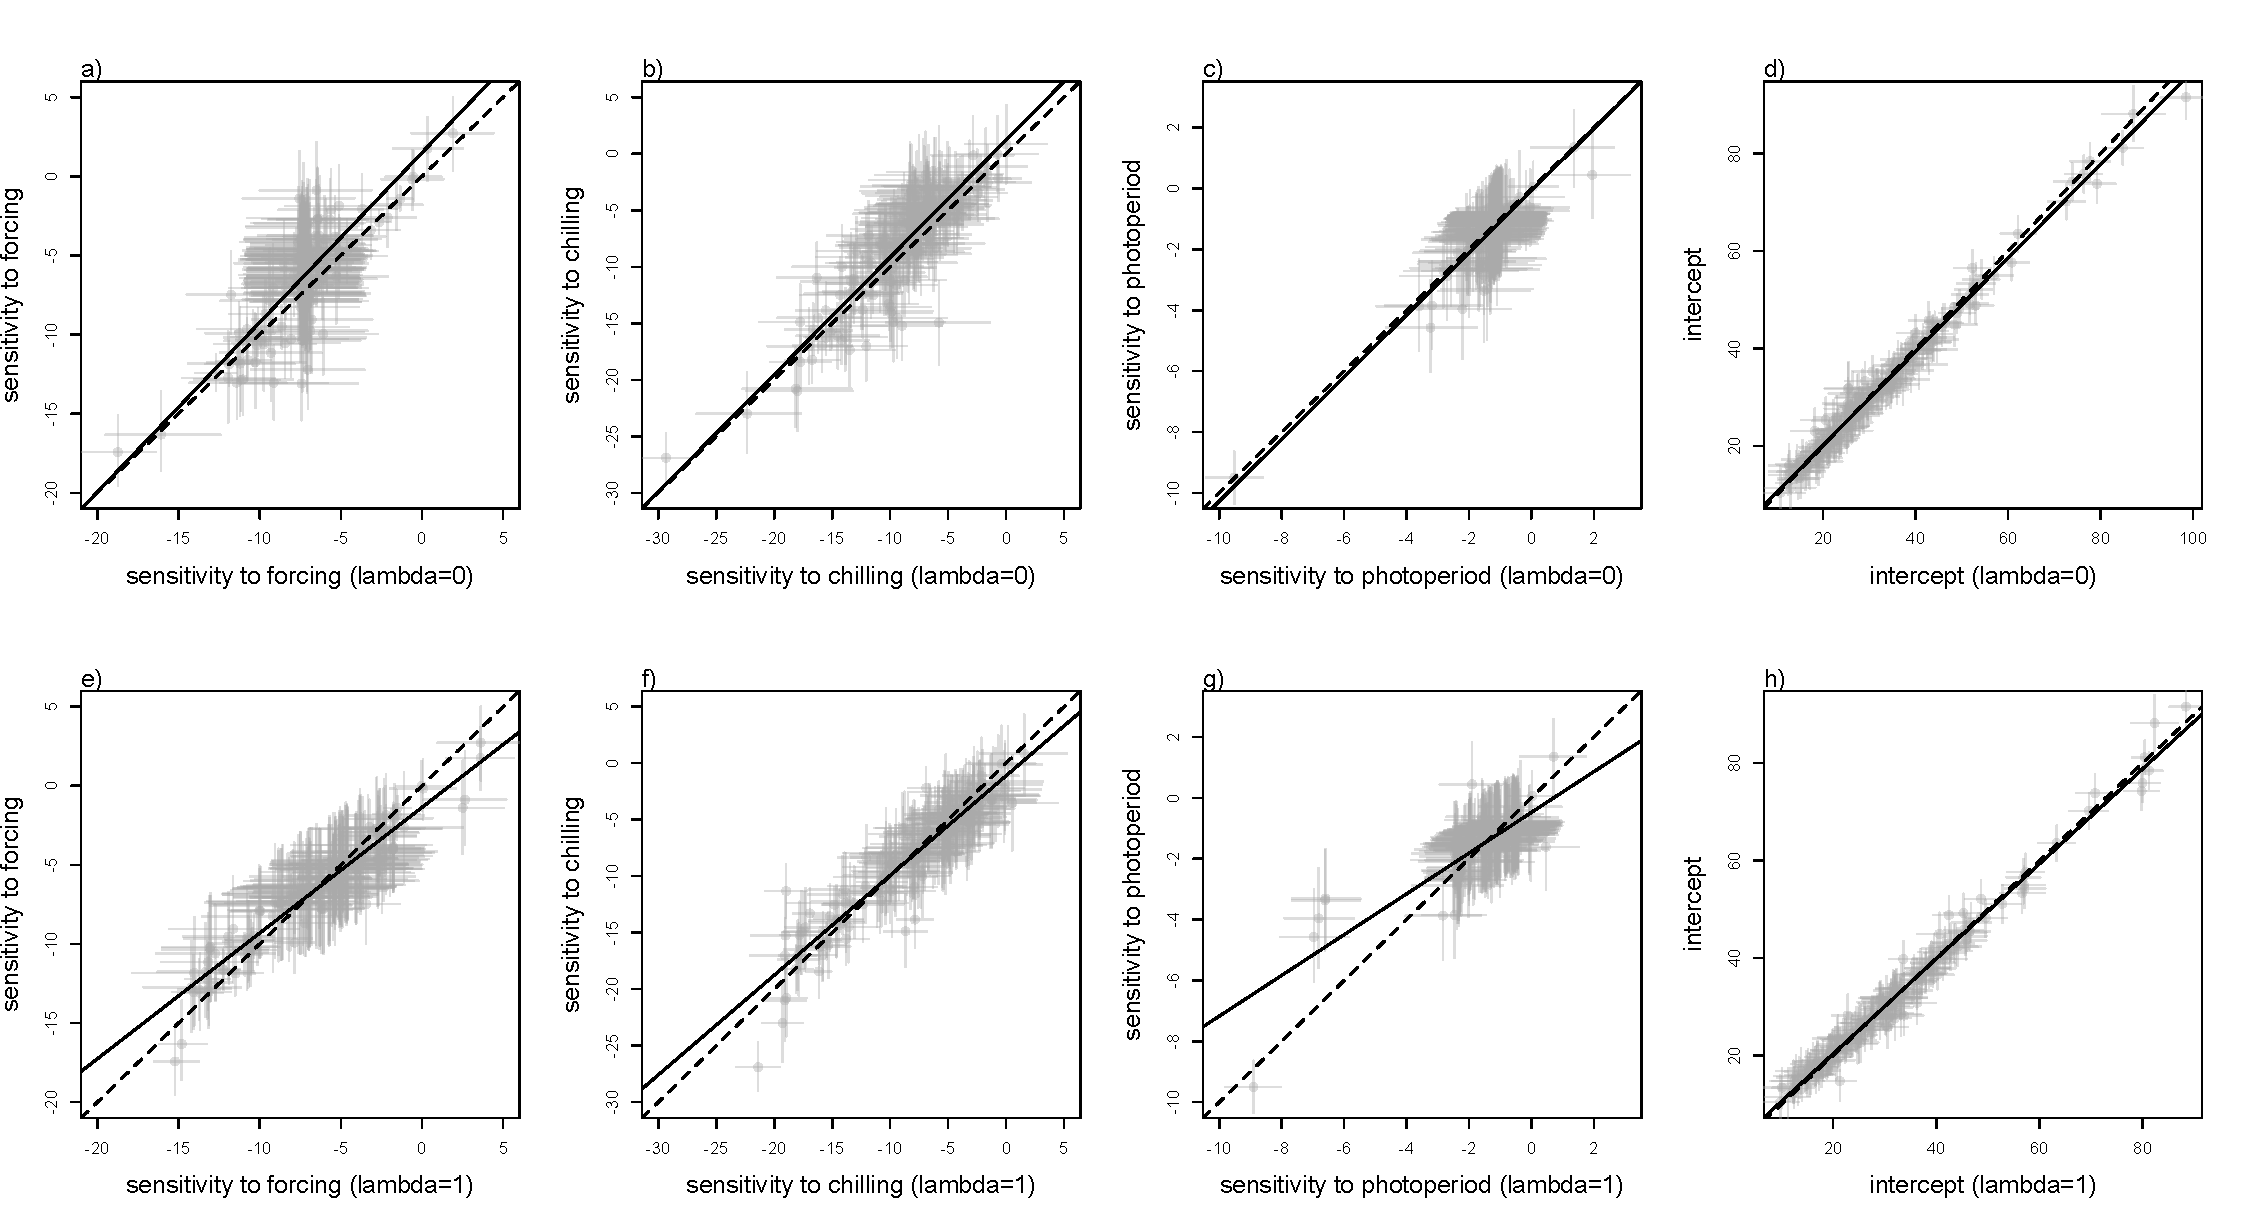
\includegraphics[width=14cm]{../../analyses/phylogeny/figures/Est_correls_vs_lamb01_angio.pdf}
  \caption{Correlations between model parameters as estimated by the full model and the models where lambda is constrained to be equal zero (upper row) or one (bottom row), for angiosperms. Panels correspond to sensitivity to forcing (a,e), to chilling (b,f), to photoperiod (c,g) and to model intercepts (d,h).}
  \label{fig:correls_angio}
  \end{center}
\end{figure}

\begin{figure} [H]
  \begin{center}
  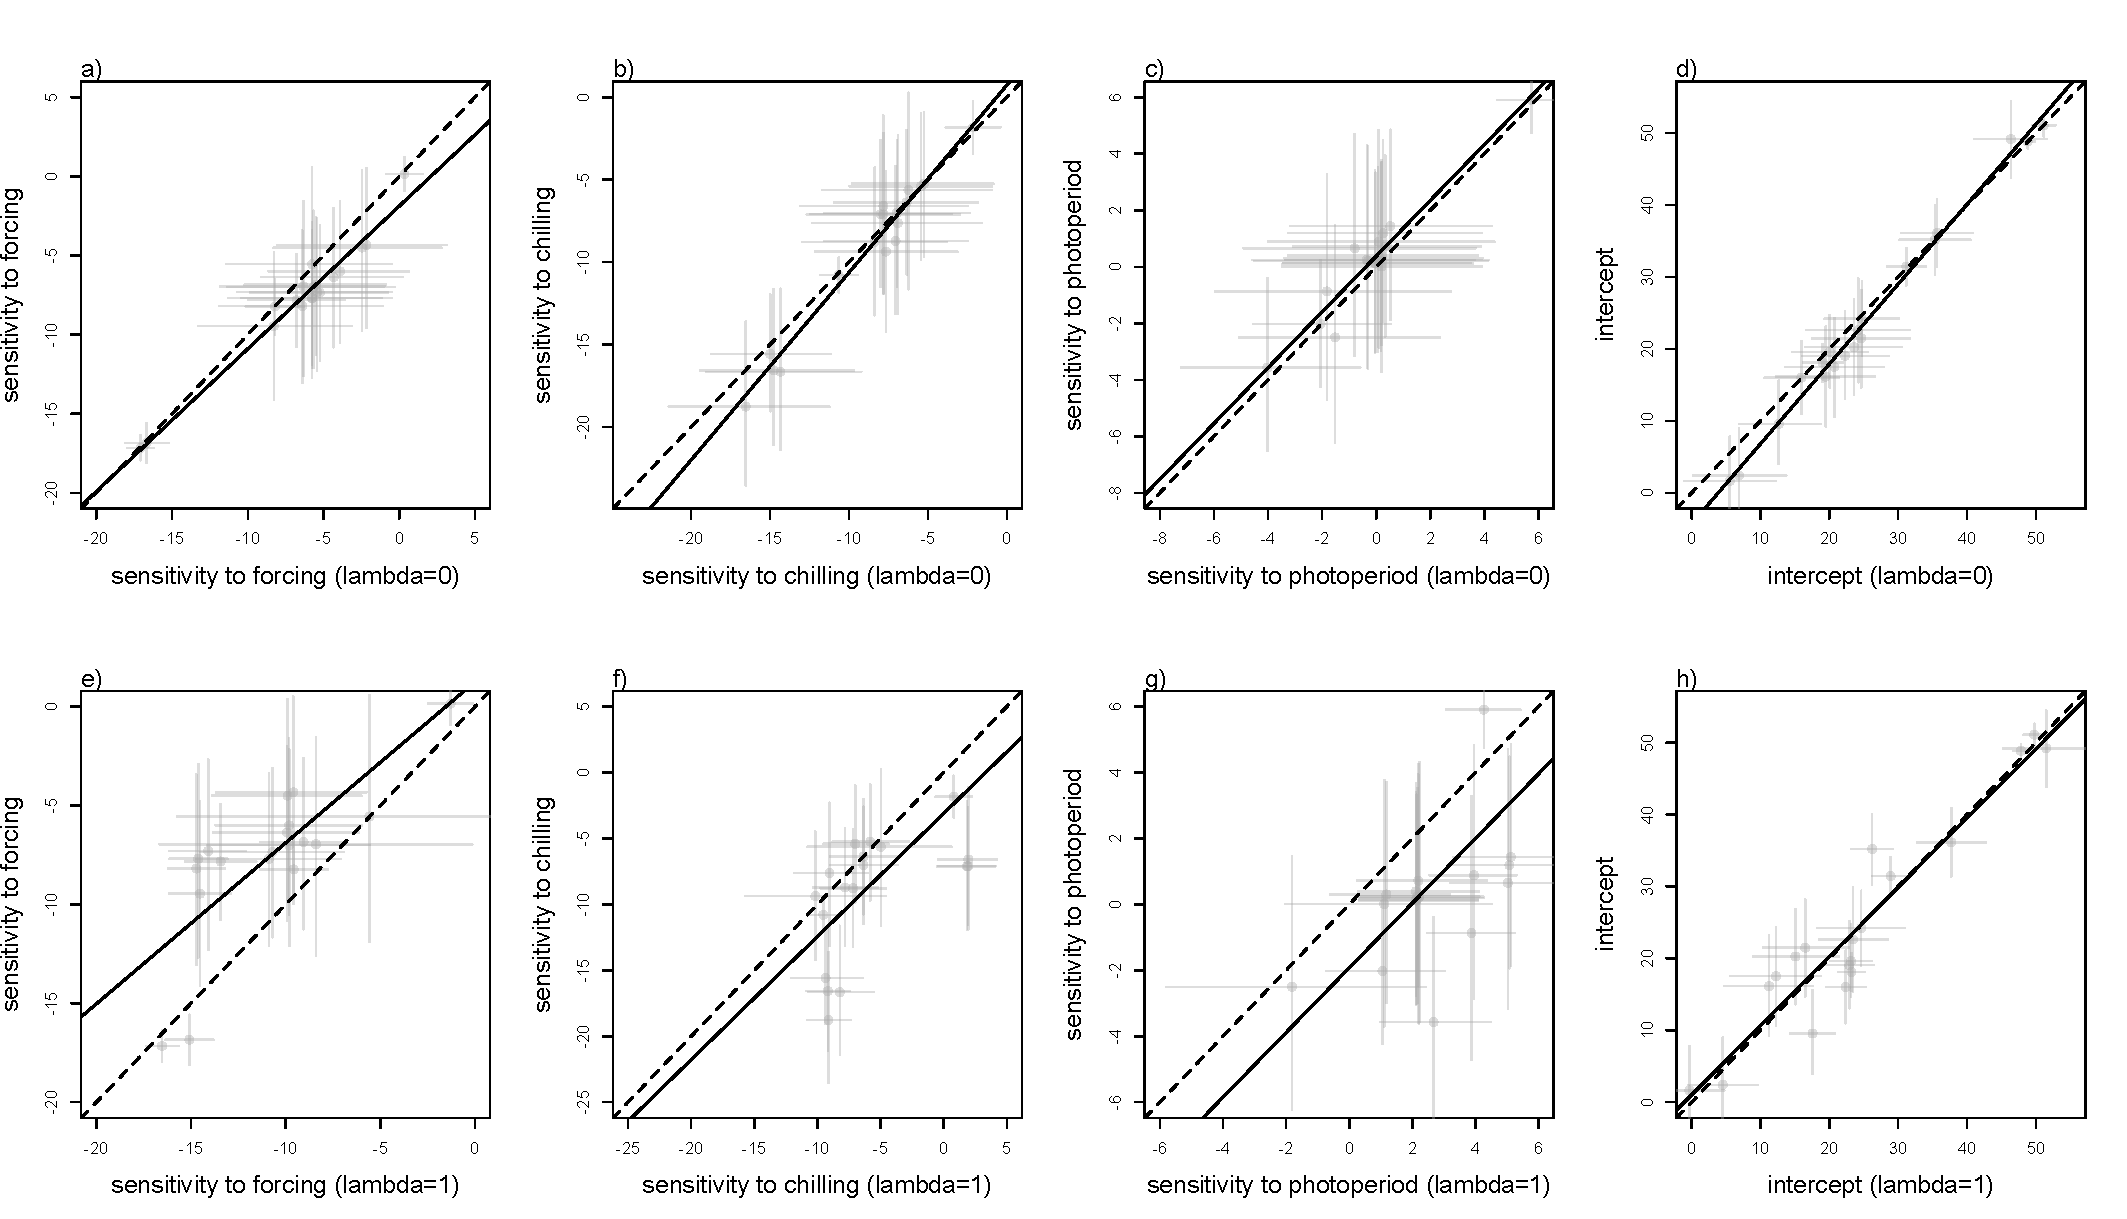
\includegraphics[width=14cm]{../../analyses/phylogeny/figures/Est_correls_vs_lamb01_gymno.pdf}
  \caption{Correlations between model parameters as estimated by the full model and the models where lambda is constrained to be equal zero (upper row) or one (bottom row), for gymnosperms. Panels correspond to sensitivity to forcing (a,e), to chilling (b,f), to photoperiod (c,g) and to model intercepts (d,h).}
  \label{fig:correls_gymno}
  \end{center}
\end{figure}



% IMC Mar21 - I'm guessing we are going to merge some of the tables below. TBD what we keep for the main text and what is sent to a supp.
\begin{table}[H]
\begin{center}
\caption{Full model parameters estimated for 192 angiosperm species.}
\begin{tabular}{@{}lcccccc@{}}
\toprule
\textbf{parameter}             & \multicolumn{1}{l}{\textbf{mean}} & \multicolumn{1}{l}{\textbf{sd}} & \multicolumn{1}{l}{\textbf{2.50\%}} & \multicolumn{1}{l}{\textbf{50\%}} & \multicolumn{1}{l}{\textbf{97.50\%}} & \multicolumn{1}{l}{\textbf{n\_eff}} \\ \midrule
$\mu_\alpha$                   & 30.57                             & 3.41                            & 23.68                               & 30.59                             & 37.14                                & 5031.19                             \\
$\mu_\beta_{forcing}$          & -5.84                             & 2.01                            & -9.72                               & -5.89                             & -1.79                                & 2374.73                             \\
$\mu_\beta_{chilling}$         & -7.19                             & 2.03                            & -11.15                              & -7.18                             & -3.18                                & 3694.93                             \\
$\mu_\beta_{photoperiod}$      & -1.37                             & 0.76                            & -2.92                               & -1.35                             & 0.14                                 & 1565.41                             \\
$\lambda_\alpha$               & 0.35                              & 0.10                            & 0.16                                & 0.34                              & 0.56                                 & 3416.51                             \\
$\lambda_\beta_{forcing}$      & 0.68                              & 0.20                            & 0.23                                & 0.71                              & 0.98                                 & 185.35                              \\
$\lambda_\beta_{chilling}$     & 0.56                              & 0.15                            & 0.25                                & 0.56                              & 0.83                                 & 738.57                              \\
$\lambda_\beta_{photoperiod}$  & 0.36                              & 0.24                            & 0.02                                & 0.33                              & 0.88                                 & 296.51                              \\
$\sigma_\alpha^2$              & 15.93                             & 1.17                            & 13.84                               & 15.85                             & 18.41                                & 2988.37                             \\
$\sigma_\beta^2_{forcing}$     & 5.84                              & 1.04                            & 4.03                                & 5.78                              & 8.15                                 & 502.74                              \\
$\sigma_\beta^2_{chilling}$    & 7.05                              & 0.87                            & 5.48                                & 7.02                              & 8.92                                 & 1026.77                             \\
$\sigma_\beta^2_{photoperiod}$ & 2.45                              & 0.41                            & 1.74                                & 2.42                              & 3.32                                 & 469.46                              \\
$\sigma_y^2$                   & 12.81                             & 0.18                            & 12.47                               & 12.80                             & 13.17                                & 4017.16                             \\ \bottomrule
\end{tabular}
\end{center}
\label{tab:modelanglamb}
\end{table}


\begin{table}[H]
 \begin{center}
\caption{Full model parameters estimated for 19 gymnosperm species.}
\begin{tabular}{@{}lcccccc@{}}
\toprule
\textbf{parameter}             & \multicolumn{1}{l}{\textbf{mean}} & \multicolumn{1}{l}{\textbf{sd}} & \multicolumn{1}{l}{\textbf{2.50\%}} & \multicolumn{1}{l}{\textbf{50\%}} & \multicolumn{1}{l}{\textbf{97.50\%}} & \multicolumn{1}{l}{\textbf{n\_eff}} \\ \midrule
$\mu_\alpha$                   & 25.75                             & 4.50                            & 16.88                               & 25.73                             & 34.73                                & 33151.86                            \\
$\mu_\beta_{forcing}$          & -5.92                             & 3.80                            & -12.97                              & -6.05                             & 1.90                                 & 16443.03                            \\
$\mu_\beta_{chilling}$         & -8.11                             & 3.63                            & -15.31                              & -8.09                             & -0.94                                & 21379.81                            \\
$\mu_\beta_{photoperiod}$      & -0.88                             & 3.33                            & -8.01                               & -0.67                             & 5.19                                 & 16301.93                            \\
$\lambda_\alpha$               & 0.47                              & 0.26                            & 0.02                                & 0.48                              & 0.90                                 & 15934.03                            \\
$\lambda_\beta_{forcing}$      & 0.36                              & 0.23                            & 0.02                                & 0.33                              & 0.84                                 & 14336.60                            \\
$\lambda_\beta_{chilling}$     & 0.32                              & 0.23                            & 0.01                                & 0.28                              & 0.82                                 & 13230.88                            \\
$\lambda_\beta_{photoperiod}$  & 0.37                              & 0.24                            & 0.02                                & 0.34                              & 0.88                                 & 11199.49                            \\
$\sigma_\alpha^2$              & 23.47                             & 6.20                            & 13.87                               & 22.59                             & 37.81                                & 18272.58                            \\
$\sigma_\beta^2_{forcing}$     & 8.89                              & 2.45                            & 4.96                                & 8.60                              & 14.51                                & 8126.51                             \\
$\sigma_\beta^2_{chilling}$    & 10.47                             & 2.66                            & 5.78                                & 10.30                             & 16.17                                & 8539.38                             \\
$\sigma_\beta^2_{photoperiod}$ & 7.18                              & 2.29                            & 3.29                                & 6.96                              & 12.25                                & 5625.69                             \\
$\sigma_y^2$                   & 15.81                             & 0.41                            & 15.04                               & 15.81                             & 16.63                                & 28640.16                            \\ \bottomrule
\end{tabular}
\end{center}
\label{tab:modelgymlamb}
\end{table}





\pagebreak
%\bibliographystyle{refs/bibstyles/amnat.bst}% 
%\bibliography{refs/phylorefs.bib}



\end{document}
